\documentclass[10pt]{beamer}

\usetheme{metropolis}
\usepackage{appendixnumberbeamer}

\usepackage{booktabs}
\usepackage[scale=2]{ccicons}
\usepackage{graphicx}
\usepackage{hyperref}
\usepackage{circuitikz}
\usepackage{pdflscape}
\usepackage{smartdiagram}

\usepackage{color}
\usepackage{listings}

\lstset{
	basicstyle=\footnotesize\ttfamily,
    keepspaces=true,
    showstringspaces=false,
    language=PHP,
    commentstyle=\ttfamily,
}

\usepackage[OT4]{polski}
\usepackage[utf8]{inputenc}

\usepackage{pgfplots}
\usepgfplotslibrary{dateplot}

\usepackage{xspace}
\newcommand{\themename}{\textbf{\textsc{metropolis}}\xspace}

\setbeamertemplate{frame footer}{}
\setbeamertemplate{frame numbering}{}

\usetikzlibrary{shapes,arrows}

\tikzstyle{decision} = [diamond, draw, fill=blue!20, 
    text width=4.5em, text badly centered, node distance=3cm, inner sep=0pt]
\tikzstyle{block} = [rectangle, draw, fill=blue!20, 
    text width=5em, text centered, rounded corners, minimum height=4em]
\tikzstyle{line} = [draw, -latex']
\tikzstyle{cloud} = [draw, ellipse,fill=red!20, node distance=3cm,
    minimum height=2em]


\title{Testy jednostkowe i behawioralne}

\subtitle{Projektowanie i programowanie systemów internetowych I}
\author{mgr inż. Krzysztof Rewak}
\date{\today}
\institute{Wydział Nauk Technicznych i Ekonomicznych \\ Państwowa Wyższa Szkoła Zawodowa im. Witelona w Legnicy}

\begin{document}

\maketitle

\begin{frame}{Plan prezentacji}
  \setbeamertemplate{section in toc}[sections numbered]
  \tableofcontents[hideallsubsections]
\end{frame}


\begin{frame}{Jak ugryźć testowanie?}
	Testy są \textbf{niezbędną} częścią procesu wytwarzania oprogamowania.
\end{frame}

\begin{frame}{Jak ugryźć testowanie?}
	Trudno sobie wyobrazić programowanie \emph{na ślepo}: tworzenie nowych funkcjonalności bez sprawdzania czy faktycznie działają.
	
	Za niedziałający program pracodawca mógłby rozwiązać umowę, klient - nie zapłacić pieniędzy, a nauczyciel - wystawić negatywną ocenę.
\end{frame}

\begin{frame}{Jak ugryźć testowanie?}
	Testy są \textbf{niezbędną} częścią procesu wytwarzania oprogamowania i wykonujemy jest bardzo często bezwiednie.
\end{frame}

\begin{frame}{Jak ugryźć testowanie?}
	\centering
	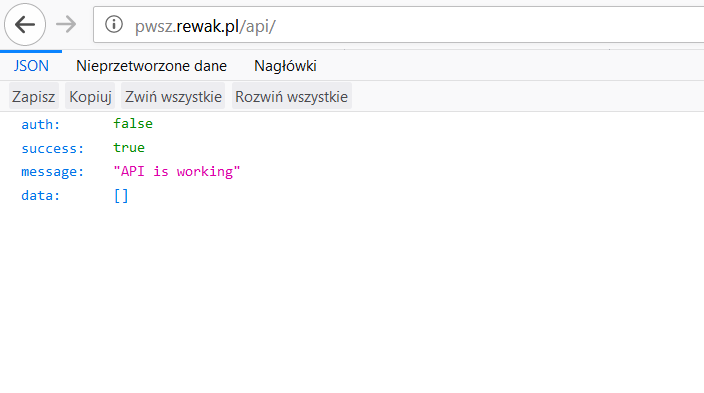
\includegraphics[width=.95\textwidth]{api2.png}
\end{frame}

\section{Testy manualne}

\begin{frame}{Testowanie manualne}
	Testowanie manualne jest \emph{najprostszym} sposobem testowania oprogramowania i polega na ręcznym przeklikaniu aplikacji w celu znalezienia błędów.
\end{frame}

\begin{frame}{Testowanie manualne}
	\centering
	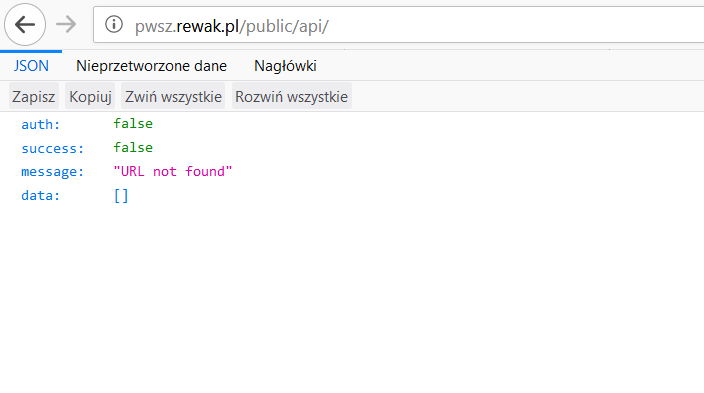
\includegraphics[width=.95\textwidth]{api.png}
\end{frame}

\begin{frame}{Testowanie manualne}
	Problem pojawi się oczywiście w momencie, w którym zwiększy się liczba testów potrzebnych do sprawdzenia stanu aplikacji.
\end{frame}

\begin{frame}{Testowanie automatyczne}
	Stąd wziął się pomysł na \textbf{testowanie automatyczne}.
\end{frame}

\section{Testy jednostkowe}

\begin{frame}{Testy jednostkowe}
	Test jednostkowy sprawdza czy metoda lub funkcja wykonuje się w oczekiwany sposób. Sprawdzenie warunku nazywa się \textbf{asercją}.
\end{frame}

\begin{frame}[fragile]{Co testować?}
	Oto prosta metoda dzieląca liczbę przez liczbę:

\begin{lstlisting}
public static function
divide(float $dividend, float $divisor): float {
    if($divisor == 0) {
        throw new DoNotDivideByZeroException();
    }
    
    return $dividend / $divisor;
}
\end{lstlisting}
\end{frame}

\begin{frame}[fragile]{Jak testować?}
	Czy to jest wystaczający test?

\begin{lstlisting}
public function testDividingFunction(): void {
    $this->assertEquals(Math::divide(1.0, 2.0), 0.5);
}
\end{lstlisting}
\end{frame}

\begin{frame}[fragile]{Jak testować?}
	A to?
	
\begin{lstlisting}
public function testDividingFunction(): void {
    $this->assertEquals(Math::divide(1.0, 2.0), 0.5);
    $this->assertEquals(Math::divide(4.0, 2.0), 2.0);
}
\end{lstlisting}
\end{frame}

\begin{frame}[fragile]{Jak testować?}
	A może to?
	
\begin{lstlisting}
public function testDividingFunction(): void {
    $this->assertEquals(Math::divide(1.0, 2.0), 0.5);
    $this->assertEquals(Math::divide(4.0, 2.0), 2.0);
    $this->expectException(DoNotDivideByZeroException::class);
    Math::divide(1.0, 0.0);
}
\end{lstlisting}
\end{frame}

\begin{frame}[fragile]{Jak testować?}
	A gdyby tak...?
	
\begin{lstlisting}
public function testDividingFunction(): void {
    $this->assertEquals(Math::divide(1.0, 2.0), 0.5);
    $this->assertEquals(Math::divide(4.0, 2.0), 2.0);
    $this->assertNotEquals(Math::divide(2.0, 4.0), 1.0);
    $this->expectException(DoNotDivideByZeroException::class);
    Math::divide(1.0, 0.0);
}
\end{lstlisting}
\end{frame}

\begin{frame}[fragile]{Jak testować?}
	A co, jeżeli przekażemy zmianną typu \texttt{int}?
	
	A co, jeżeli podzielimy coś, co powinno zwrócić na przykład 3.(3)?
	
	A co, jeżeli...?
\end{frame}

\begin{frame}{Testy jednostkowe w praktyce}
	Jedna asercja na test czy wiele na funkcjonalność? Dobrą praktyką jest testowanie osobno, jednakże wybór może zostać wymuszony (w obie strony) przez specyfikę projektu.
\end{frame}

\begin{frame}{Testy jednostkowe w praktyce}
	Ogólnie przyjęte zasady mówią, że testować jednostkowo powinno się wszystkie publiczne metody klas w projekcie.
	
	Oczywiście stuprocentowe pokrycie testami może być czymś do czego warto dążyć, ale niektóre metody (chociażby proste settery i gettery) zwyczajnie nie potrzebują być testowane.
\end{frame}

\begin{frame}{Kiedy testować?}
	Testy jednostkowe najlepiej uruchamiać... zawsze. 
	
	Przy commitach, przy merge requestach, przy wdrożeniu. Najlepiej zautomatyzować proces wdrożeniowy w taki sposób, aby przejście przez wszystkie testy było obowiązkowe przed wprowadzeniem zmian na serwerze.
\end{frame}

\begin{frame}{Mockowanie}
	Czasami chcemy przetestować coś, co jest uwikłane w sieć zależności. Wyobraźmy sobie serwis, w którym używana jest klasa pobierająca listę użytkowników z bazy danych i wysyłają im newsletter poprzez mejla.
	
	Karygodnym błędem byłoby przetestowanie tego na danych produkcyjnych i wysłanie każdemu mejla przy każdym teście, prawda?
\end{frame}

\begin{frame}{Mockowanie}
	Dlatego do testowania wygodne jest wykorzystanie wzorca projektowego odwracania zależności. Wówczas można z poziomu testu wywołać potrzebny serwis z \emph{mockiem} klasy pobierającej dane czy wysyłającej mejle.
	
	Taki \emph{mock} (ang. atrapa) będzie symulowanym odzwieciedleniem wymaganej funkcjonalności. Przykładowo gdy \texttt{users.all()} odwołuje się do bazy danych i zwraca tablicę użytkowników, mockowany obiekt \texttt{users} klasy \texttt{MockUsers} może dla metody \texttt{all()} wypisać zahardkodowane dane.
\end{frame}

\begin{frame}[fragile]{Mockowanie}	
	Które rozwiązanie będzie lepsze do mockowania obiektów?
\begin{lstlisting}
public function send(): void {
    $mailer = new Mailer;
    $mailer->send();
}
\end{lstlisting}

	czy może:

\begin{lstlisting}
public function send(Mailer $mailer): void {
    $mailer->send();
}
\end{lstlisting}

	czy może:

\begin{lstlisting}
public function send(MailerInterface $mailer): void {
    $mailer->send();
}
\end{lstlisting}
\end{frame}

\begin{frame}[fragile]{Pro-tip}
	Ostrzeżenie: młodych programistów kusi czasami testowanie losowanych danych:
	
\begin{lstlisting}
public function testDividingFunction(): void {
    for($i = 0; $i < 100; $++) {
        $a = rand(); $b = rand();
	$this->assertEquals(Math::divide($a, $b), $a / $b);
    }
}
\end{lstlisting}

	Istotą testowania jest sprawdzenie jak program zadziała w kontrolowanych warunkach. Jeżeli programista chce sprawdzić inne warunki, musi stworzyć nowy test z konkretnymi wartościami.

\end{frame}

\begin{frame}{Czym testować?}
	\begin{itemize}
	\item PHP: PHPUnit, PHP Unit Testing Framework, Behat
	\item JavaScript: Mocha, Unit.js
	\item .NET: csUnit, NUnit, Visual Studio Unit Testing Framework
	\item Python: Doctest, pytest
	\item Java: JUnit
	\item go: go test
	\item Ruby: RSpec
	\item C++: CppUnit
	\end{itemize}
\end{frame}
	
\section{Testy behawioralne}

\begin{frame}{Testy behawioralne}
	Czasami zdarza się, że klient aktywnie bierze udział przy tworzeniu projektu. Oczywiście nie programuje, ale przecież to od niego zależy co będzie wykonywała opracowywana aplikacja.
	
	Klient powinien znać domenę projektu, a więc powinien znać wszystkie realia środowiskowe.
\end{frame}

\begin{frame}{Testy behawioralne}
	O ileż prostsze byłoby programowanie, gdyby klient zamiast opowiadania o wymaganiach, mógłby rozpisać scenariusze zachowań aplikacji?
\end{frame}

\begin{frame}{Testy behawioralne}
	Problem ten pomaga rozwiązać idea testów behawioralnych.
\end{frame}

\begin{frame}[fragile]{\texttt{news.feature}}	
	Przykładowy test może wyglądać następująco:
	
\begin{lstlisting}
Scenario: Checking if retrieving newsreel returns correct result:
  When a client requests "/api/news" with "GET" method
  Then "200" status code should be received
  And proper response array should be received
  And response array should have success status
  And response array should have empty message
  And response array should not have empty data array
  And there should be "3" news entries
  And received news should be arranged in chronological order
\end{lstlisting}
\end{frame}

\begin{frame}[fragile]{\texttt{Context.php}}	
	Przykładowo realizacja zdania:
	
\begin{lstlisting}
Then "200" status code should be received
\end{lstlisting}

	może wyglądać następująco:
	
\begin{lstlisting}
public function
statusCodeShouldBeReceived(string $statusCode): void {
  $responseStatusCode = (string) $this->response->getStatusCode();
  PHPUnit::assertEquals($responseStatusCode, $statusCode);
}
\end{lstlisting}
\end{frame}

\begin{frame}{Testy behawioralne}
	Korzytając ze słów kluczowych \texttt{Given}, \texttt{When} i \texttt{Then} można stworzyć \emph{historyjki} opisujące każdy przypadek omawianej aplikacji.
\end{frame}

\begin{frame}{Testy behawioralne}
	Testy behawioralne \emph{pod spodem} korzystają z asercji znanych z testów jednostkowych, jednakże są wygodniejsze do planowania i czytania dla osób nietechnicznych lub nie będących programistami. Język Gherkin jest uniwersalny i może być stosowany do kontekstów napisanych w Ruby (Cucumber), PHP (Behat), Java (YatSpec/Concordion), .NET (SpecFlow) i innych.
\end{frame}

\section{Selenium}

\begin{frame}{Testy regresyjne}
	Przedstawione przykłady świetnie się wpisują do testowania backendu.
	
	A co jeżeli chcemy przeklikać frontend naszej aplikacji?
\end{frame}

\begin{frame}{Testy regresyjne}
	Z pomocą przychodzi Selenium, czyli narzędzie do automatyzacji testów. Pozwala ono na \emph{nagranie} interakcji z interfejsem aplikacji i następnie powtarzanie go w ramach testowania funkcjonalności.
\end{frame}

\begin{frame}{Testy regresyjne}
	\centering
	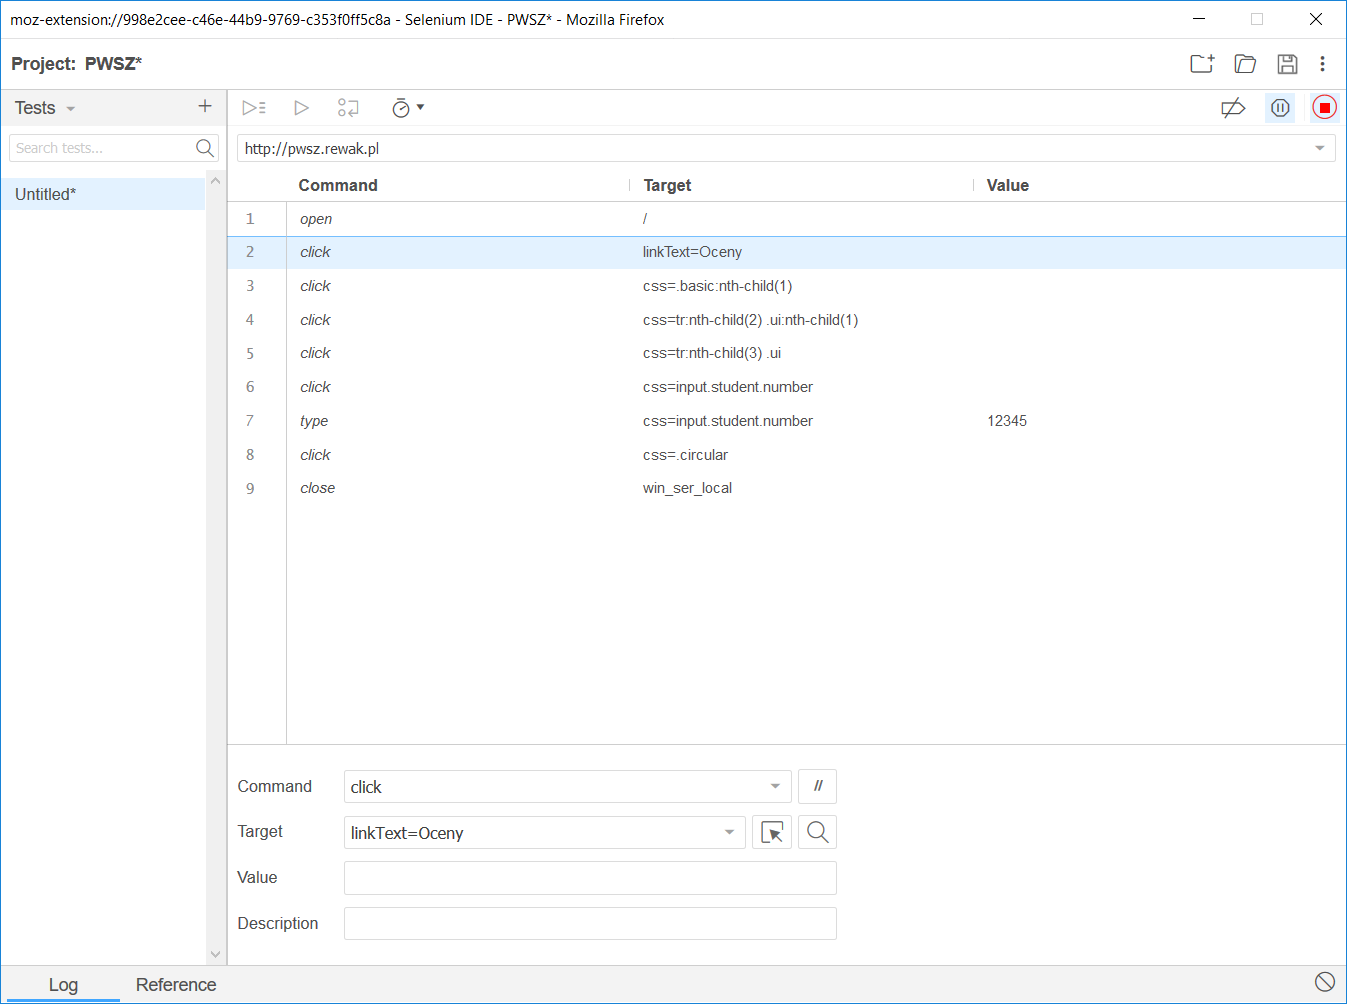
\includegraphics[width=.95\textwidth]{selenium.png}
\end{frame}

\begin{frame}{Testy regresyjne}
	Kiedy przyda się taka możliwość testowania?
	
	Na pewno w momencie, w którym wprowadzamy zmiany, które mogą rzutować na inne części aplikacji. Nawet stuprocentowe pokrycie testami jednostkowymi nie zagwarantuje tego, że wszystko od strony użytkownika będzie działało poprawnie.
\end{frame}

\section{Test Driven Development}

\begin{frame}[fragile]{TDD}
	TDD to jeden z elementów tzw. \emph{exterme programming}, czyli metodologii wytwarzania oprogamowania z którą każdy powinien się zapoznać w którymś momencie kariery.
	
	\textbf{Test Driven Development}, czyli mniej więcej \emph{programowanie prowadzone testami}, to idea wedle której testy powinny zostać napisane przed rozpoczęciem pracy nad daną funkcjonalnością.
\end{frame}

\begin{frame}{Co?}
	\centering
	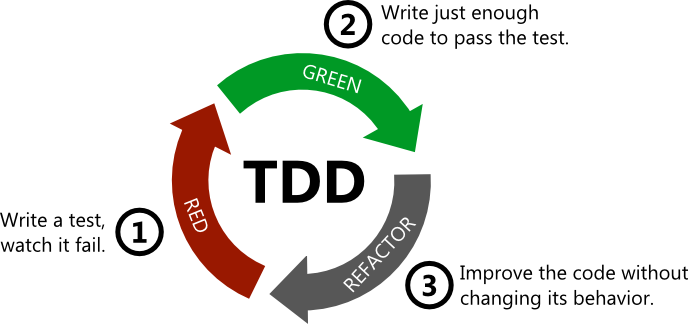
\includegraphics[width=.95\textwidth]{tdd.png}
	
	\ \\
	
	źródło: https://medium.com/pacroy/test-driven-development-tdd-resource-site-tdd-pacroy-com-a02e02396f32
\end{frame}

\begin{frame}{TDD w trzech krokach}
	Najpierw piszemy test opsiujący funkcjonalność którą chcemy dodać. Uruchamiamy go i otrzymujemy serię błędów, ponieważ nie stworzyliśmy jeszcze kodu, który miałby się uruchomić poprawnie.
\end{frame}

\begin{frame}{TDD w trzech krokach}	
	Następnie dopisujemy funkcjonalność. Pod koniec tego kroku uprzednio napisany test powinien zakończyć sie sukcesem.
\end{frame}

\begin{frame}{TDD w trzech krokach}
	Wówczas dokonujemy \emph{refactoru}, czyli poprawiamy wszystko, co nie wiąże się bezpośrednio z działaniem funkcjonalnym, ale może poprawić szeroko rozumianą jakość kodu.
\end{frame}

\begin{frame}{TDD w trzech krokach}
	Wówczas dokonujemy \emph{refactoru}, czyli poprawiamy wszystko, co nie wiąże się bezpośrednio z działaniem funkcjonalnym, ale może poprawić szeroko rozumianą jakość kodu.
\end{frame}

\section{Podsumowanie}

\begin{frame}{Bibliografia i ciekawe źródła}
  
	\begin{thebibliography}{9}
	
		\bibitem{rewak}
		Krzysztof Rewak,
		\textit{Projektowanie i programowanie obiektowe},
		materiały do zajęć laboratoryjnych
	
	\end{thebibliography}

\end{frame}

\appendix

\begin{frame}[standout]
	Pytania?
\end{frame}

\begin{frame}{}

	Kod prezentacji dostępny jest w repozytorium git pod adresem \texttt{https://bitbucket.org/krewak/pwsz-ppsi} \\ \ \\

	\begin{figure}
		\centering
		\href{https://bitbucket.org/krewak/pwsz-ppsi}{
			
\includegraphics[width=.15\textwidth]{../_template/bitbucket.png}
		}
	\end{figure}
	
	Wszystkie informacje dot. kursu dostępne są pod adresem \texttt{http://pwsz.rewak.pl/kursy/4} \\ \ \\

	\begin{figure}
		\centering
		\href{http://pwsz.rewak.pl/kursy/3}{
			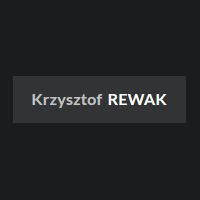
\includegraphics[width=.15\textwidth]{../_template/rewak.png}
		}
	\end{figure}

\end{frame}

\end{document}
